\documentclass[tikz,border=10pt]{standalone}
\begin{document}
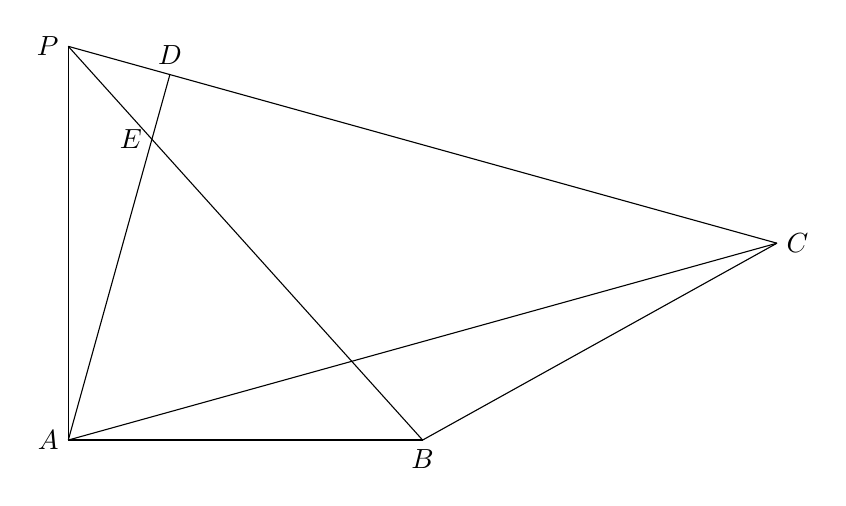
\begin{tikzpicture}
    \coordinate (P) at (0, 5);
    \coordinate (A) at (0, 0);
    \coordinate (B) at (4.5, 0);
    \coordinate (C) at (9, 2.5);
    \coordinate (D) at (1.29, 4.64);
    \coordinate (E) at (1.06, 3.82);

    \draw (P) -- (A);
    \draw (A) -- (B);
    \draw (B) -- (C);
    \draw (C) -- (P);
    \draw (P) -- (B);
    \draw (A) -- (C);
    \draw (A) -- (D);

    \node[left] at (P) {$P$};
    \node[left] at (A) {$A$};
    \node[below] at (B) {$B$};
    \node[right] at (C) {$C$};
    \node[above] at (D) {$D$};
    \node[left] at (E) {$E$};
\end{tikzpicture}
\end{document}
